\documentclass[a5paper]{article}
\usepackage[a5paper, top=8mm, bottom=8mm, left=8mm, right=8mm]{geometry}

\usepackage{polyglossia}
\setdefaultlanguage[babelshorthands=true]{russian}

\usepackage{fontspec}
\setmainfont{FreeSerif}
\newfontfamily{\russianfonttt}[Scale=0.7]{DejaVuSansMono}

\usepackage[font=scriptsize]{caption}

\usepackage{amsmath}
\usepackage{amssymb,amsfonts,textcomp}
\usepackage{xcolor}
\usepackage{array}
\usepackage{hhline}
\usepackage{cite}

\usepackage[hang,multiple]{footmisc}
\renewcommand{\footnotelayout}{\raggedright}

\PassOptionsToPackage{hyphens}{url}\usepackage[xetex,linktocpage=true,plainpages=false,pdfpagelabels=false]{hyperref}
\hypersetup{colorlinks=true, linkcolor=blue, citecolor=blue, filecolor=blue, urlcolor=blue, pdftitle=1, pdfauthor=, pdfsubject=, pdfkeywords=}

\usepackage{tabu}

\usepackage{graphicx}
\usepackage{indentfirst}
\usepackage{multirow}
\usepackage{subfig}
\usepackage{footnote}
\usepackage{minted}

\newcommand{\attribution}[1] {
\vspace{-2mm}\begin{flushright}\begin{scriptsize}\textcolor{gray}{\textcopyright\, #1}\end{scriptsize}\end{flushright}
}

\sloppy
\pagestyle{plain}

\title{Высокоуровневая многопоточность}
\author{Юрий Литвинов\\\small{y.litvinov@spbu.ru}}

\date{28.09.2021}

\begin{document}

\maketitle
\thispagestyle{empty}

\section{Введение}

В этой лекции пойдёт речь о высокоуровневых механизмах работы с многопоточными программами. На самом деле, низкоуровневыми потоками через класс Thread прикладные программисты практически никогда не пользуются, да и низкоуровневые примитивы синхронизации типа AutoResetEvent-ов в реальном коде можно встретить весьма редко. Некоторые авторы указвают, что вообще, если в вашей программе есть \mintinline{csharp}|new Thread()|, ваша программа уже устарела.

Что предлагается взамен --- проектировать многопоточные программы не в терминах потоков, а в терминах задач, которые могут исполняться параллельно. Тогда эти задачи можно будет раскидать по потокам, которыми управляют библиотеки, а не создавать потоки вручную. В стандартной библиотеке .NET есть механизм управления потоками, который всё сделает за вас (ThreadPool). Более того, есть и высокоуровневые языковые средства (async/await), которые используют ThreadPool и позволяют без нужды вообще не думать о параллельности и асинхронности. Программист может писать программу практически как обычную последовательную, а компилятор делает так, что всё работает хорошо.

Тем не менее, знать про низкоуровневые потоки всё равно нужно, потому что все высокоуровневые механизмы многопоточного и асинхронного исполнения используют Thread и все низкоуровневые штуки, что были на предыдущих парах. Если про них не знать, можно получать внезапные дедлоки в async-методах, или делать программу существенно менее параллельной, чем она могла бы быть. Этим часто страдают даже опытные разработчики.

\section{Пул потоков}

\subsection{Foreground- и Background-потоки}

Начнём мы со всё ещё довольно низкоуровневой конструкции, которая, тем не менее, уже существенно облегчает жизнь --- пула потоков. Но для начала введём понятия Foreground- и Background-потоков.

Когда все Foreground-потоки завершили работу, рантайм останавливает все Background-потоки и заканчивает работу приложения, в этом, собственно, и есть их различие. Background-потоки можно понимать как вспомогательные, состояние которых на момент окончания работы некритично. Хороший способ прострелитьь себе ногу --- создать foreground-поток, который бы бесконечно что-то делал, и забыть о нём. Причём, поскольку работа с консолью или UI живут в своём потоке, вы можете закрыть окно приложения, оно как будто закроется, но работу не завершит (будет висеть в списке задач в Task Manager или аналогичных штуках). И будет держать запущенным процесс, а следовательно, и все связанные с ним ресурсы (открытые файлы, в частности). Печаль в том, что Thread создаёт потоки по умолчанию как Foreground-потоки, так что если не делать им Join, может такое случиться.

Однако есть и обратный способ прострелить себе ногу: создать background-поток и не дать ему доработать. Вот пример (заодно показывающий, как переключать режимы потоков):

\begin{minted}{csharp}
var t = new Thread(Worker);
t.IsBackground = true;
t.Start();
Console.WriteLine("Returning from Main");
\end{minted}

Worker может вообще никогда не получить управление, потому что планировщик решит дать основному потоку доработать, а он закончит исполнение целого приложения.

\subsection{Пул потоков}

Пул потоков --- это набор заранее созданных Background-потоков, которые готовы принимать задачи на исполнение. Причём, это довольно умная штука, которая управляется .NET-машиной и принимает во внимание оборудование и операционную систему, на которой она запущена. Концептуально у пула потоков есть единая очередь, куда можно поставить задачу (в виде лямбда-функции, ссылки на метод и т.д.), и он вернёт объект типа Task, который позволяет вызывающему следить за статусом задачи и забрать результат, когда он будет готов (или заблокироваться и подождать результата). То есть Task --- это что-то вроде представителя в ``главном'' потоке задачи, делающейся в одном из потоков пула. При этом, разумеется, если получать результат нам не надо, Task можно не создавать, как в примере ниже:

\begin{minted}{csharp}
public static void Main() {
    Console.WriteLine("Главный поток: ставим задачу в очередь");
    ThreadPool.QueueUserWorkItem(ComputeBoundOp, 5);
    Console.WriteLine("Главный поток: занимаемся своими делами...");
    Thread.Sleep(10000);  // Симуляция работы в главном потоке
    Console.WriteLine("Нажмите <Enter>, чтобы закрыть программу...");
    Console.ReadLine();
}

private static void ComputeBoundOp(Object state) {
    Console.WriteLine($"Внутри ComputeBoundOp: state={state}");
    Thread.Sleep(1000);  // Симуляция работы в потоке из пула
}
\end{minted}

ThreadPool.QueueUserWorkItem принимает саму операцию и ``состояние'' --- произвольный объект (типа Object), который может использоваться для передачи параметров в операцию (если их надо много, то передавайте структуру, но вообще обычно явно параметры не передают, потому что есть замыкания). Свободный поток из пула подхватывает операцию и начинает её исполнять. Если все потоки заняты, пул может запустить ещё несколько потоков, если сочтёт нужным --- запускать потоков больше, чем ядер процессора, может быть осмысленно, если потоки заблокировались на длительной операции типа сетевого запроса, и ядра простаивают. Если задач мало, пул автоматически останавливает лишние потоки до некоторого минимума, который автоматически определяет по количеству доступных .NET-машине ядер.

Пул потоков редко используется в прикладных программах напрямую, зато используется повсеместно в реализации более высокоуровневых вещей, таких как async/await.

\subsection{Отмена операций}

Задачи из пула можно прерывать до их завершения, но с некоторыми ограничениями, присущими вообще всем операциям отмены и прерывания потоков в многопоточном программировании. .NET использует принцип \textit{коллаборативной} отмены операции --- ``рабочему'' потоку и ``главному'' потоку доступен булевый флажок, который ``главный'' поток выставляет при необходимости отмены, а ``рабочий'' время от времени проверяет. Если флажок выставлен, рабочий поток должен корректно завершиться. При этом если рабочий поток не в состоянии проверить флажок (например, заблокировался на длительной операции, задедлочился, просто что-то считает), прервать его таким способом будет невозможно. Почему так --- если просто насильно прервать исполнение задачи в потоке, она может оставить систему в неконсистентном состоянии. И беда даже не в том, что, например, поток не успеет дописать сохранение в файл или как-то ещё испортить данные (что само по себе очень не очень), но в том, что поток мог в это время захватить какой-нибудь мьютекс, и если его просто взять и прервать, он не сможет никогда его отдать, так что дальше задедлочится и вся остальная система. 

Кстати, есть более грубый способ прервать поток --- через метод Thread.Interrupt. Interrupt выбросит в прерываемом потоке ThreadInterruptedException из заблокировавшей поток операции (Sleep, Wait и т.п.), что, скорее всего, остановит поток, при этом корректно исполнив все finally и отдав все lock-и (что, конечно, не гарантирует, что вернут все захваченные мьютексы, но всё же). Тем не менее, поток вправе поймать это исключение и продолжить работать, так что даже это не гаранирует остановку потока. Более сильное средство --- Thread.Abort, но им лучше не пользоваться вообще (и оно не работает в .NET Core). Thread.Abort выкидывает исключение из любой операции, а не только операции длительного ожидания, так что может, например, прервать исполнение статического конструктора и сломать всю систему. И тоже не гарантирует завершение потока.

Собственно, тот самый булевый флажок для коллаборативной отмены в .NET называется CancellationToken. Есть ещё CancellationTokenSource --- часть ``флажка'', остающаяся в основном потоке. Из CancellationTokenSource можно получить CancellationToken, отдать его в рабочий поток, и при необходимости отмены вызвать CancellationTokenSource.Cancel(). Это изменит связанный с ним CancellationToken, рабочий поток это увидит и, будем надеяться, остановится. Вот пример:

\begin{minted}{csharp}
public static void Main() {
    var cts = new CancellationTokenSource();
    ThreadPool.QueueUserWorkItem(o => Count(cts.Token, 1000));
    Console.ReadLine();
    cts.Cancel();
    Console.ReadLine();
}

private static void Count(CancellationToken token, int countTo) {
    for (int count = 0; count < countTo; count++) {
        if (token.IsCancellationRequested) {
            break;
        }
        Thread.Sleep(200); 
    }
}
\end{minted}

\subsection{Task}

Теперь немного подробнее о классе Task --- как гвоорилось выше, ``представителе'' задачи из параллельного потока в потоке, её вызвавшем. Подобная Task вещь в Java называется Future, а в C++ это даже пара классов std::future/std::promise --- что хорошо отражает назначение этой концепции, ``значение, которое будет доступно когда-то в будущем''. 

В .NET Task, помимо хранения значения, может сам и запускать вычисления на потоке из пула. Например,

\begin{minted}{csharp}
ThreadPool.QueueUserWorkItem(ComputeBoundOp, 5);

new Task(ComputeBoundOp, 5).Start();

Task.Run(() => ComputeBoundOp(5));
\end{minted}

--- это эквивалентные строки кода. Task.Run удобнее, поэтому вот как раз его используют в прикладных программах, чтобы быстро что-нибудь сделать параллельно.

Task тоже используется для реализации высокоуровневой функциональности, например, все асинхронные методы возвращают именно Task, из которого можно получить значение, дождавшись его вручную, а можно подождать с помощью ключевого слова await.

Вот более типичный пример использования Task:

\begin{minted}{csharp}
private static int Sum(int n) {
    int sum = 0;
    for (; n > 0; n--)
        sum += n;
    return sum;
}
...
Task<int> t = new Task<int>(n => Sum((int)n), 1000000000);
t.Start();
// Тут занимаемся своими делами, Sum считается в отдельном потоке из пула
t.Wait();  // t.Result сам делает Wait(), так что тут это только для иллюстрации
Console.WriteLine("Сумма: " + t.Result);
\end{minted}

Тут как раз делаются какие-то длительные вычисления, мы их запускаем в потоке из пула (хотя, как видите, ThreadPool тут нигде не упоминается, Task про него знает и использует именно его), пока вычисления идут, мы можем заниматься какой-то полезной работой, затем дождаться результата и показать его пользователю с помощью метода Task.Result. Если результат уже готов, Result его тут же возвращает, если нет, блокирует вызвавший его поток до тех пор, пока он не будет готов.

Task-и, разумеется, можно отменять, и, разумеется, тоже с помощью CancellationToken-ов. Например, Sum можно было бы модифицировать так:

\begin{minted}{csharp}
private static int Sum(CancellationToken ct, int n) {
    int sum = 0;
    for (; n > 0; n--) {
        ct.ThrowIfCancellationRequested();
        sum += n;
    }
    return sum;
}
\end{minted}

Метод ThrowIfCancellationRequested кидает OperationCanceledException в основной поток при обращении к результату (на самом деле, AggregateException с OperationCanceledException), и это считается более идеологически правильно, чем проверять IsCancellationRequested вручную --- ThrowIfCancellationRequested одновременно и закончит работу нашего потока, и даст вызывающему знать, что нам не дали досчитаться и значению из Result нельзя доверять (на самом деле, он даже не даст вызываающему ничего из Result получить). Вручную через IsCancellationRequested это тоже можно сделать, но надо бросить исключение самим, а зачем, если за нас это уже сделано.

\subsection{TaskScheduler}

TaskScheduler --- это класс, представляющий прослойку между Task и пулом потоков, которая отвечает за то, где и когда исполняется Task. TaskScheduler может использоваться для того, чтобы исполнять Task-и не на пуле потоков вообще, и даже если пул потоков нас устраивает, TaskScheduler умеет более тонко настраивать исполнение Task-ов, например, завадавая, когда вызывать continuation Task-а (то есть следующий Task, использующий результат предыдущего). По умолчанию TaskScheduler ставит Task-и на исполнение в пул потоков, но может быть полезно, например, continuation для какой-нибудь длинной задачи исполнить не на потоке из пула, а в текущем потоке:

\begin{minted}{csharp}
Task<int> t = Task.Run(() => Sum(cts.Token, 20000), cts.Token);
t.ContinueWith(task => Text = "Result: " + task.Result,
        CancellationToken.None,
        TaskContinuationOptions.OnlyOnRanToCompletion,
        TaskScheduler.FromCurrentSynchronizationContext());
\end{minted}

Здесь выполняется какое-то долгое вычисление и мы хотим показать его результаты в форме в GUI. Модифицировать элементы GUI принципиально можно только из потока GUI, так что потоки из пула в принципе никаких свойств пользовательского интерфейса менять не могут (и программа упадёт, как только они попытаются). Поэтому мы делаем хитро: мы основные вычисления делаем в потоке на пуле с помощью Task-а t, и вешаем ему continuation (с помощью метода Task.ContinueWith, который на самом деле тоже возвращает Task). continuation должен исполниться в основном потоке, поэтому мы передаём ему в качестве шедулера результат вызова \mintinline{csharp}|TaskScheduler.FromCurrentSynchronizationContext()|, который вернёт шедулер, запускающий Task в том потоке, откуда был создан этот шедулер (то есть, в нашем случае, в GUI-потоке). Теперь, когда t исполнится на одном из потоков из пула, она захочет вызвать ContinueWith, создастся Task и отправится в очередь GUI-потоку, и если он будет свободен (то есть ждать в цикле обработки событий, что GUI-потоки в основном и делают), исполнит её и спокойно обновит UI.

На самом деле, TaskScheduler --- это очень мощный инструмент управления многопоточным исполнением, но в прикладном коде используется по полной довольно редко (как и все очень мощные инструменты), поэтому про него тут не очень подробно. Метод FromCurrentSynchronizationContext, тем не менее, рекомендую запомнить, когда мы дойдём до продвинутых UI-приложений, он нам понадобится.

\section{async/await}

\subsection{Паттерн Begin.../End...}

Task и пул потоков хороши для дорогих по времени операций, которые надо считать на нескольких ядрах сразу, но начинают страдать, если параллельность требуется для длительных асинхронных операций, состоящих по большей части из ожидания. Поток, вставший на асинхронной операции, не может исполнять задачи дальше, пул вынужден создавать новые потоки, что трудоёмко и требует системных ресурсов, так что все преимущества пула сходят на нет. На самом деле, обычно программы большую часть времени занимаются ожиданием, и когда это параллельное ожидание сразу многих событий, просто создавать задачи и кидать их в пул на исполнение становится крайне неэффективно. Синхронная операция чтения (которую можно выполнять в отдельном потоке) работает примерно так:

\begin{center}
    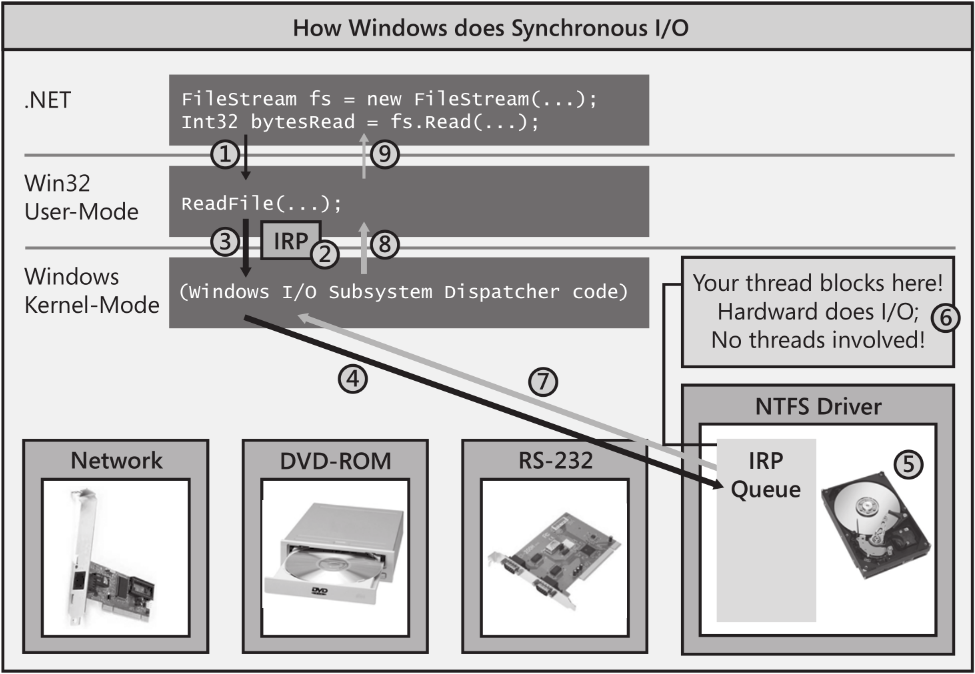
\includegraphics[width=0.5\textwidth]{windowsSynchronousIO.png}

    \begin{footnotesize}(Рисунок из Jeffrey Richter. CLR via C\#)\end{footnotesize}
\end{center}

Когда мы делаем вызов синхронной операции чтения из файла, она на самом деле дёргает библиотеку WinAPI, которая переключает программу в режим ядра, которая блокирует вызвавший поток (это делает планировщик), формирует I/O Request Packet для драйвера и ставит его в очередь. Драйвер передаёт команду диску, диск грузит требуемые данные в память (без помощи процессора, это делает микросхема Direct Memory Access), после чего дёргает драйвер (через аппаратное прерывание), тот будит поток и возвращает управление.

В .NET практически с самого начала был и асинхронный интерфейс для операций ввода-вывода, построенный на коллбэках --- точнее, паттерне Begin.../End.... Работает это так:

\begin{center}
    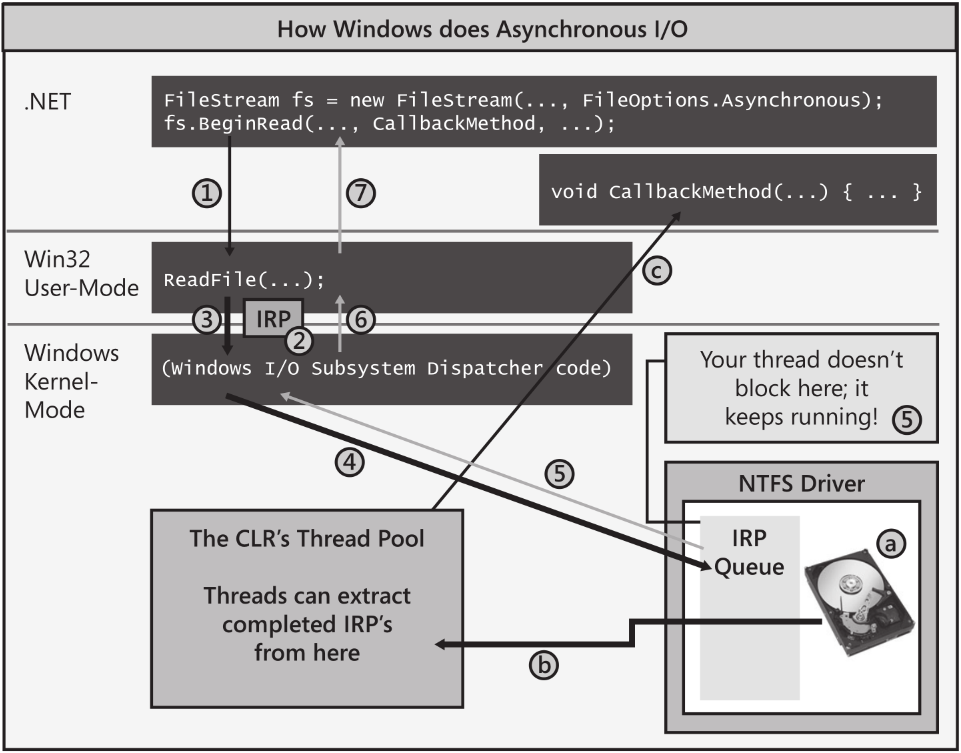
\includegraphics[width=0.5\textwidth]{windowsAsynchronousIO.png}

    \begin{footnotesize}(Рисунок из Jeffrey Richter. CLR via C\#)\end{footnotesize}
\end{center}

\mintinline{csharp}|Begin...()| инициирует операцию, принимая колбэк, где можно использовать \mintinline{csharp}|End...()|, чтобы получить результат. \mintinline{csharp}|Begin...()| точно так же дёргает функцию WinAPI, которая формирует IRP, отдаёт его драйверу, но не ждёт исполнения его на устройстве, а тут же возвращает управление. Основной поток может продолжать работу, при этом данные ещё не готовы. А когда операция заканчивается, драйвер дёргает операционную систему, та вызыввает коллбэк .NET-машины, которая находит в пуле потоков незанятый поток и вызывает в нём переданный в \mintinline{csharp}|Begin...()| коллбэк. При этом, пока диск копирует данные в память, буквально ни один поток этим не заблокирован.

\subsection{async/await}

До C\# 5 (то есть до 2012 года) все так и жили, было написано довольно много кода в таком стиле, поэтому \mintinline{csharp}|Begin...()| и \mintinline{csharp}|End...()| можно встретить много где в стандартной библиотеке и в документации. Тем не менее, сейчас этими методами пользоваться не надо, есть новая модель асинхронного программирования: async/await. Работает оно как-то так:

\begin{center}
    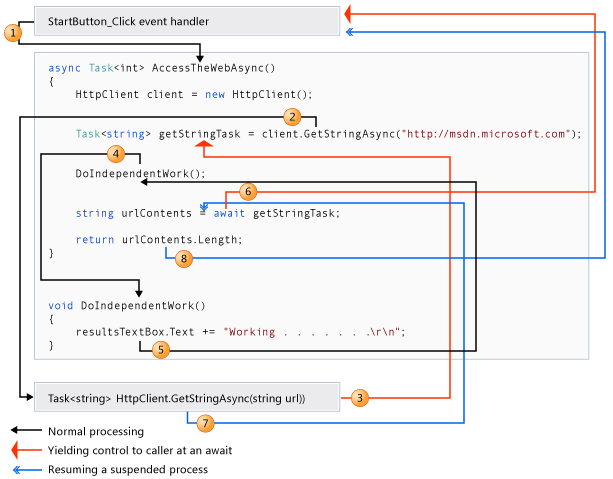
\includegraphics[width=0.6\textwidth]{asyncAwait.png}

    \begin{footnotesize}(Рисунок из \href{https://msdn.microsoft.com/library/hh191443(vs.110).aspx}{MSDN})\end{footnotesize}
\end{center}

В C\# добавилось два новых ключевых слова, \mintinline{csharp}|async|, означающий, что метод, им помеченный, является асинхронным, и \mintinline{csharp}|await|, позволяющий неблокирующим образом дождаться результата асинхронного вызова. Звучит сложно, но работает довольно просто: \mintinline{csharp}|await| возвращает управление вызывающему до тех пор, пока асинхронная операция не закончится, а когда она заканчивается, исполнение продолжается со строки с \mintinline{csharp}|await|. 

Если посмотреть на картинку, то оно работает так. Допустим, у нас есть кнопка, по нажатию на которую мы хотим получить содержимое какой-то веб-страницы (что требует сетевых запросов, а это долгая операция). Помечаем её обработчик как \mintinline{csharp}|async|. Делаем асинхронный вызов, получая в качестве результата Task. При этом операция начинается в отдельном потоке (на пуле, конечно же), а Task, как обычно, представляет собой ``значение, которое будет доступно когда-то в будущем'' (стартовать Task вручную не нужно, кстати). Дальше мы можем ещё что-нибудь полезное поделать, но когда всё сделали, делаем \mintinline{csharp}|await| на этот Task. И вот тут происходит магия --- если результат ещё не готов, исполнение нашего метода прерывается и он возвращает управление выше по стеку (почти как будто ему return сделали). Если выше по стеку цикл обработки событий, то начинает работать он, он может обрабатывать какие-то другие события (у нас вот кнопка, значит, есть UI, и пока асинхронная операция не закончилась, UI может обрабатывать пользовательский ввод, так что интерфейс не виснет). Когда операция наконец заканчивается, в цикл обработки событий ставится задача продолжить вычисление со строки с \mintinline{csharp}|await|. Оно продолжается как обычно, когда наш поток готов эту задачу выполнить, и метод возвращает управление как обычно.

Разумеется, для реализации такой штуки требуется серьёзная поддержка со стороны компилятора. Внутри класса, в котором есть асинхронные методы, генерируется конечный автомат, который запоминает, на каком \mintinline{csharp}|await| мы сейчас находимся, и реагирует на события типа окончания асинхронных операций, вызывая при переходах действия между \mintinline{csharp}|await|-ами. На самом деле, подобную штуку мы уже видели --- это \mintinline{csharp}|yield return|, и действительно, теоретические корни у механизма async/await, как и у yield-ов, растут из понятия ``сопрограмма'' (которое было популярно в своё время, аж в 1960-х, но потом забыто и только недавно вернулось в мэйнстримные языки). Понимать реализацию сопрограмм в C\# можно как Task-и с набором continuation-ов: делай всё до первого await-а, запусти асинхронную операцию, и когда она закончится, вызови continuation, в котором делай всё до следующего await-а или return. Причём, если в рассмотренном нами примере обработчик вызывался в GUI-шном потоке, в общем случае continuation-ы могут исполняться на первом подвернувшемся потоке из пула, так что один метод с await-ами может последовательно исполняться в нескольких разных потоках! Если понимать происходящее как цепочку вызовов continuation-ов, то это становится более понятно. Кроме того, через continuation-ы честно распространяются исключения, так что можно писать try-catch даже с await-ами внутри, и всё нормально поймается, даже несмотря на то, что у каждого потока свой стек и исключение, брошенное в одном потоке, будет поймано в другом. Программист об этом может даже не думать. Собственно, поэтому async/await и стал так популярен, и стал одной из ключевых особенностей языка C\# (кстати, в C++ или Java нет ничего подобного).

Вот небольшой пример того, как это в коде выглядит:

\begin{minted}{csharp}
private static async Task<int> Method1Async() { ... }
private static async Task<string> Method2Async() { ... }

private static async Task<string> MyMethodAsync(int argument) {
    int local = argument;
    try {
        int result1 = await Method1Async();
        for (int x = 0; x < 3; x++) {
            string result2 = await Method2Async();
        }
    }
    catch (Exception) { Console.WriteLine("Catch"); }
    return "Done";
}
\end{minted}

Обратите внимание, что метод, в котором есть await, сам должен быть async (и тогда его тоже можно await-ить) --- ему надо временно отдавать управление, надо, чтобы было куда. Ещё обратите внимание, что await вполне может быть в цикле, тогда просто несколько раз будет выполняться ожидание и всё будет работать как и в последовательном случае. Ну и исключения, понятное дело, ловятся как обычно.

\subsection{Особенности async/await}

async-метод может возвращать только \mintinline{csharp}|Task|, \mintinline{csharp}|Task<T>| или \mintinline{csharp}|void|, другие типы возвращаемого значения --- ошибка компиляции. Думаю, что понятно, почему --- он не может вернуть значение напрямую, потому что оно может быть ещё не готово. При этом \mintinline{csharp}|void| в принципе не позволяет получить результат и даже дождаться окончания асинхронной операции, поэтому весьма нишевая штука --- используется для асинхронных обработчиков событий или для асинхронного Main. Причём, и то и другое kind of хак: асинхронные обработчики событий должны возвращать \mintinline{csharp}|void|, потому что переопределяют библиотечные обработчики событий, которые синхронные (и были написаны ещё до всего этого безумия), так что если они бы возвращали Task, типы бы не сошлись. Асинхронный Main звучит здорово, но на самом деле ничего не делает (просто ждёт результата асинхронной операции) --- выше по стеку Main-а никакого цикла обработки событий нет, там только рантайм .NET-а, так что можно сделать обычный синхронный Main, а вместо await написать .Result, и будет то же самое. Но асинхронный Main типа красивее.

Кстати, await можно ждать не только результата асинхронного метода, но и вообще любой Task, хоть обычный Task.Run, который мы научились писать в начале лекции. И наоборот, никто не заставляет вас await-ить все async-методы, можно принять из него Task и продолжить работу. А потом воспользоваться обычным Task.Result и другими методами Task-а (это самый обычный Task). При этом вызов Result у асинхронного метода заставляет его исполниться синхронно --- поток блокируется на Result до тех пор, пока асинхронная операция не закончится. Что убивает все преимущества async/await-ов, поэтому за такое надо сразу увольнять, но я часто встречал такое в продакшн-коде. Общее правило таково, что если метод асинхронный, то и все вызывающие его вверх по стеку до самого конца должны быть асинхронными, если нет веских причин для обратного\footnote{А они бывают --- например, когда мы используем асинхронные методы только для распараллеливания: запускаем асинхронно сразу пачку методов, потом синхронно ждём их всех. Но зачем?}.

Ещё, кстати, стоит заметить, что \mintinline{csharp}|await| как бы снимает с типа возвращаемого значения Task. Например, если асинхронный метод возвращает \mintinline{csharp}|Task<int>|, то \mintinline{csharp}|await| на этот метод вернёт \mintinline{csharp}|int|. И если \mintinline{csharp}|await| случайно забыть, то асинхронный метод вернёт \mintinline{csharp}|Task<T>|, что, если вы любите \mintinline{csharp}|var|-ы, может пройти незамеченным для компилятора. Это ещё один способ прострелить себе ногу --- внимательно следите, где вы хотите посчитанный результат, а где ссылку на задачу.

Да, и всё это работает только с .NET 4.5 и выше, хотя это, наверное, не так критично, потому что вряд ли кто использует в качестве целевого более старую версию. Если только вы не пишете для Windows XP, там .NET есть только до версии 4, и всё это так сходу не заработает (поможет библиотека Microsoft.BCL, впрочем, которая предоставляет весь необходимый рантайм для более старых версий .NET. Но в любом случае компилятор должен быть C\# 5 или свежее).

\subsection{async и исключения}

Ещё одна небольшая тонкость связана с тем, когда именно бросаются исключения при выполнении асинхронной операции. Операция выполняется в отдельном потоке, поэтому исключение надо как-то ``доставить'' в вызывающий поток, и делает это Task.Result, или \mintinline{csharp}|await|:

\begin{minted}{csharp}
static async Task ThrowExceptionAsync() {
    await Task.Delay(TimeSpan.FromSeconds(1));
    throw new InvalidOperationException("Всё плохо");
}

static async Task TestAsync() {
    // Исключение не бросается, а сохраняется в Task-е
    Task task = ThrowExceptionAsync();
    try {
        // Исключение бросается при выполнении await (или обращении к Result)
        await task;
    } catch (InvalidOperationException) {
        // Исключение ловится здесь как обычно
    }
}
\end{minted}

\subsection{Async-методы в стандартной библиотеке}

Асинхронные методы нет смысла делать асинхронными, если в них нет ни одного \mintinline{csharp}|await|-а, что приводит к некоторой вариации проблемы курицы и яйца --- где-то должны быть асинхронные методы, которые не содержат в себе других асинхронных методов, но при этом сами асинхронны. Первый источник таких ``базовых'' методов --- это стандартная библиотека. Там асинхронных методов довольно много, практически ко всем длительным операциям есть асинхронный интерфейс (более того, в .NET Core работает \textbf{только} асинхронный интерфейс ко многим вещам, если его специально не попросить). Вот некоторые полезные примеры:

\begin{itemize}
    \item \mintinline{csharp}|System.IO.Stream| и потомки: \mintinline{csharp}|ReadAsync|, \mintinline{csharp}|WriteAsync|, \mintinline{csharp}|FlushAsync|, \mintinline{csharp}|CopyToAsync| --- файловый (точнее, потоковый, не только файловый) ввод/вывод;
    \item \mintinline{csharp}|System.IO.TextReader| и потомки: \mintinline{csharp}|ReadAsync|, \mintinline{csharp}|ReadLineAsync|, \mintinline{csharp}|ReadToEndAsync|, \mintinline{csharp}|ReadBlockAsync| --- высокоуровневый файловый ввод, с понятием ``строка'';
    \item \mintinline{csharp}|System.IO.TextWriter| и потомки: \mintinline{csharp}|WriteAsync|, \mintinline{csharp}|WriteLineAsync|, \mintinline{csharp}|FlushAsynс| --- то же самое с выводом;
    \item \mintinline{csharp}|System.Net.Http.HttpClient|: \mintinline{csharp}|GetAsync|, \mintinline{csharp}|GetStreamAsync|, \mintinline{csharp}|GetByteArrayAsync|, \mintinline{csharp}|PostAsync|, \mintinline{csharp}|PutAsync|, \mintinline{csharp}|DeleteAsync| и т.д. --- работа с сетью;
    \item \mintinline{csharp}|System.Net.WebRequest| и потомки: \mintinline{csharp}|GetRequestStreamAsync| и \mintinline{csharp}|GetResponseAsynс| --- более высокоуровневая работа с сетью;
    \item \mintinline{csharp}|System.Data.SqlClient.SqlCommand|: \mintinline{csharp}|ExecuteDbDataReaderAsync| --- работа с базами данных.
\end{itemize}

\subsection{Способ получить дедлок с async}

Теперь можно посмотреть на ещё один способ всё испортить, а именно получить самый настоящий дедлок, используя только async/await. Рассмотрим такой пример кода:

\begin{minted}{csharp}
private sealed class MyWpfWindow : Window {
    public MyWpfWindow() { Title = "WPF Window"; }

    protected override void OnActivated(EventArgs e) {
        string http = GetHttp().Result; // Синхронно вызываемся
        base.OnActivated(e);
    }

    private async Task<String> GetHttp() {
        HttpResponseMessage msg = 
                await new HttpClient().GetAsync("http://google.com/");
        return await msg.Content.ReadAsStringAsync();  // Никогда не дойдём сюда
    }
}
\end{minted}

Это какое-то графическое приложение, написанное на библиотеке WPF (про которую речь пойдёт далее, но это не так важно, рассуждения применимы ко всем GUI-приложениям). У нас есть обработчик OnActivated, который вызывается при появлении окна на экране, он синхронный. В нём мы вызываем метод GetHttp и, поскольку обработчик синхронный, берём его Result, в надежде, что метод рано или поздно отработает (а мы пока подождём), мы получим результат и присвоим его куда-нибудь. В асинхронном методе GetHttp мы делаем запрос на получение содержимого веб-страницы, ждём его await-ом, потом асинхронно же получаем результат и возвращаем его. Что на самом деле происходит --- мы вызываем GetHttp, он начинает исполняться синхронно (обрратите внимание, асинхронный метод до первого await работает как обычный), выполняет асинхронный запрос и встаёт на await, возвращая управление в GetHttp. GetHttp блокируется на Result. Операция заканчивается, рантайм добавляет потоку в очередь continuation, который должен будет проинициализировать msg и исполнить ReadAsStringAsync. Но, поскольку это GUI-приложение, этот continuation по умолчанию шедулится на GUI-поток (такое умолчание принято, чтобы не надо было всегда думать о TaskScheduler при написании GUI-приложений). А GUI-поток заблокирован ожиданием результата этого continuation-а. Оба куска кода ждут друг друга, дедлок. 

В GUI-приложениях особенно опасайтесь вызывать Result-ы.

\subsection{Несколько полезных методов Task}

Ещё несколько полезных штук:

\begin{itemize}
    \item Подождать сколько-то миллисекунд:
    \begin{minted}{csharp}
await Task.Delay(delay);
    \end{minted}
    Это очень похоже на Thread.Sleep, но правильный и асинхронный (который не блокирует поток).

    \item Сразу же вернуть результат:
    \begin{minted}{csharp}
// Возвращает Task, который исполняется синхронно
Task.FromResult(13);
    \end{minted}
    Это полезно, если у вас есть синхронный API, который вы не можете/не хотите переписывать под  асинхронность, но хотите использовать его в контексте, где ожидаются асинхроннные методы (например, в тестах).
\end{itemize}

Ещё есть методы, позволяющие организовать несколько Task-ов в одну и ждать их одновременно. Первый --- Task.WhenAll:

\begin{minted}{csharp}
int[] results = await Task.WhenAll(task1, task2, task3);
\end{minted}

Возвращает результат, когда готовы все результаты всех Task-ов, при этом результатом будет массив из результатов соответствующих Task-ов. Раз так, то все Task-и ддолжны возвращать результат одного типа.

Task.WhenAny возвращает результат, когда выполниась хотя бы одна из переданных ему задач. В отличие от Task.WhenAll возвращает не ответ, а саму выполнившуюся задачу (если их несколько закончилось одновременно, то какую-нибудь). Из этой задачи можно потом получить Result, и он гарантированно будет доступен.

Например, это можно использовать, чтобы просто организовать таймаут для асинхронной операции:

\begin{minted}{csharp}
static async Task<string> DownloadStringWithTimeout(string uri)
{
    using (var client = new HttpClient())
    {
        var downloadTask = client.GetStringAsync(uri);
        var timeoutTask = Task.Delay(3000);
        var completedTask = await Task.WhenAny(downloadTask, timeoutTask);
        if (completedTask == timeoutTask)
            return null;
        return await downloadTask;
    }
}
\end{minted}

\section{Task Parallel Library}

Есть ещё более высокоуровневые механизмы распараллеливания, один из них --- Task Parallel Library, или TPL. Эта библиотека предназначена прежде всего для распараллеливания вычислительно сложных операций, в отличие от async/await, ориентированных на ввод/вывод и долгое ожидание. TPL поставляется с .NET начиная с .NET 4.0, так что отдельно качать её не надо. Так же, как и остальные механизмы, она использует ThreadPool для выполнения Task-ов, но вот разбиение вычисления на Task-и, размещение их на пуле и синхронизацию она берёт на себя, так что программисту достаточно всего одной строчки кода для эффективного распараллеливания. TPL, пожалуй, самый удобный способ делать что-то в несколько потоков одновременно.

Например, если у нас есть цикл, в котором делаются какие-то не связанные задачи:

\begin{minted}{csharp}
for (int i = 0; i < 1000; i++) DoWork(i);
\end{minted}

Здесь прямо просится распараллеливание, и его очень легко добиться:

\begin{minted}{csharp}
Parallel.For(0, 1000, i => DoWork(i));
\end{minted}

Но обратите внимание, что задачи должны не зависеть друг от друга и не иметь зависимых друг от друга побочных эффектов --- за кажущейся простотой всё ещё скрываются все неприятности параллельного программирования, которые мы до этого обсуждали.

Или вот пример более ``тактического'' распараллеливания, когда у нас есть несколько методов, которые могут параллельно работать:

\begin{minted}{csharp}
Parallel.Invoke(
    () => Method1(),
    () => Method2(),
    () => Method3());
\end{minted}

Прерывание операций поддержано в двух вариантах --- изнутри, когда само вычисление понимает, что дальше считать нет смысла, или извне, через CancellationToken. Вот пример прерывания изнутри, через параметр state, который передаётся в лямбду Parallel.ForEach и которым можно управлять вычислением:

\begin{minted}{csharp}
void InvertMatrices(IEnumerable<Matrix> matrices)
{
    Parallel.ForEach(matrices, (matrix, state) => {
        if (!matrix.IsInvertible)
            state.Stop();
        else
            matrix.Invert();
    });
}
\end{minted}

Обратите внимание, что \mintinline{csharp}|state.Stop();| не означает, что вычисление прервётся немедленно, это всего лишь говорит, что задачи, которые ещё не поставились в потоки на пул и не должны быть поставлены. Те, что уже считаются, досчитаются спокойно. А поскольку Parallel.ForEach не гарантирует какого-то конкретного порядка вычислений задач, что именно будет посчитано, а что нет, предсказать заранее нельзя. Тем не менее, это полезно, чтобы избежать ненужных трат вычислительных ресурсов --- в нашем примере если хоть одна матрица необратима, обращать последовательность матриц дальше нет смысла.

А вот пример отмены через CancellationToken:

\begin{minted}{csharp}
void RotateMatrices(IEnumerable<Matrix> matrices, float degrees,
    CancellationToken token)
{
    Parallel.ForEach(matrices,
            new ParallelOptions { CancellationToken = token },
            matrix => matrix.Rotate(degrees));
}
\end{minted}

Если мы сделаем соответствующему CancellationTokenSource Cancel, то вычисление остановится по такому же принципу, что и изнутри --- кто уже начал считаться, досчитается, остальные задачи не будут поставлены на счёт.

В случае, если всё-таки задачи зависят друг от друга, нужна синхронизация. Об этом легко забыть благодаря кажущейся простоте TPL, но тем не менее:

\begin{minted}{csharp}
int InvertMatrices(IEnumerable<Matrix> matrices)
{
    int nonInvertibleCount = 0;
    Parallel.ForEach(matrices, matrix =>
    {
        if (matrix.IsInvertible) {
            matrix.Invert();
        } else {
            Interlocked.Increment(ref nonInvertibleCount);
        }
    });
    return nonInvertibleCount;
}
\end{minted}

Тут мы хотим обратить матрицы, которые можно обратить, и посчитать количество необратимых. Раз все задачи делаются параллельно, нам надо использовать Interlocked для увеличения счётчика, иначе будут гонки.

\section{Потокобезопасные коллекции}

В борьбе с гонками могут сильно помочь потокобезопасные коллекции из стандартной библиотеки. Они сами берут на себя вопросы доступа из разных потоков, так что могут использоваться ``как есть'', без дополнительной синхронизации, из любого многопоточного кода, как на голых Thread-ах, так и потоках из пула, PLINQ, TPL и т.п. 

Для начала важное терминологическое замечание. Потокобезопасность --- свойство кода не иметь гонок при обращении из нескольких потоков. При этом различают следующие вещи:
\begin{itemize}
    \item \textit{Thread-safe} --- возможность вызывать код из нескольких потоков;
    \item \textit{Reentrant} --- возможность вызывать код из нескольких потоков, если каждый вызов использует свои данные (например, функция, добавляющая элеемнт в список прекрасно параллельно работает для разных списков);
    \item Весь thread-safe код reentrant, но не наоборот.
\end{itemize}

Обратите внимание, что в документации по стандартной библиотеке практически везде написано, кто Thread-safe, кто Reentrant, а кто нет. При этом все коллекции, которыми мы пользовались до этого (\mintinline{csharp}{List<T>}, \mintinline{csharp}{Dictionary<K, V>} и т.д.) \textbf{не потокобезопасны}.

\subsection{Немутабельные коллекции}

Самый простой способ обеспечить потокобезопасность базируется на принципе ``Нет изменяемого состояния --- нет гонок''. Поэтому в стандартной библиотеке есть целый набор \textit{немутабельных} коллекций:

\begin{itemize}
    \item \mintinline{csharp}{ImmutableStack<T>}
    \item \mintinline{csharp}{ImmutableQueue<T>}
    \item \mintinline{csharp}{ImmutableList<T>}
    \item \mintinline{csharp}{ImmutableHashSet<T>}
    \item \mintinline{csharp}{ImmutableSortedSet<T>}
    \item \mintinline{csharp}{ImmutableDictionary<K, V>}
    \item \mintinline{csharp}{ImmutableSortedDictionary<K, V>}
\end{itemize}

Делают они то же, что и обычные, и думаю, что по названиям понятно, кто что, но их нельзя менять. Единожды заполненная элементами, коллекция всё своё время жизни останется такой, какой была, поэтому её можно смело отдавать другим потокам и работать с ней без синхронизаций. Чтение из таких коллекций потокобезопасно, а запись просто невозможна. 

Но, казалось бы, невозможность добавить в коллекцию элемент --- это такое себе свойство коллекций, как с ними работать-то? На самом деле, методы изменения коллекции есть, просто они возвращают новую коллекцию, оставляя старую неизменной. Например, с немутабельным списком можно работать так:

\begin{minted}{csharp}
var list = ImmutableList<int>.Empty;
list = list.Insert(0, 13);
list = list.Insert(0, 7);

// Пишет "7", затем "13".
foreach (var item in list)
    Console.WriteLine(item);

list = list.RemoveAt(1);
\end{minted}

Казалось бы, это может привести к очень неэффективным операциям добавления/удаления и явно приведёт к перерасходу памяти, но нет, немутабельные коллекции устроены гораздо хитрее. Вот асимптотика основных операций мутабельного и немутабельного списков:

\begin{tabu} {| X[0.9 l p] | X[1 l p] | X[1 l p] |}
    \tabucline-
    Операция     & List<T>                & ImmutableList<T>  \\
    \tabucline-
    \everyrow{\tabucline-}
    Add          & амортизированная O(1)  & O(log N)          \\
    Insert       & O(N)                   & O(log N)          \\
    RemoveAt     & O(N)                   & O(log N)          \\
    Item[index]  & O(1)                   & O(log N)          \\
\end{tabu}

Видно, что на некоторых операциях немутабельные коллекции даже выигрывают у мутабельных. И не видно, но можно поверить на слово, что дополнительной памяти тоже почти не требуется. Достигается это за счёт использования сбалансированных двоичных деревьев, разделяемых между коллекциями, так что когда мы добавляем элемент в список, коллекция на самом деле не копируется, а появляется новый элемент и правятся ссылки так, что старая коллекция всё ещё видит старое дерево, а новая коллекция --- дерево с этим элементом. Как именно это работает, подробно описано в документации, но поскольку это довольно сложно и не очень нужно, то останавливаться на этом мы не будем.

\subsection{Потокобезопасные структуры данных}

Немутабельные коллекции хороши, но бесполезны для обмена информацией между потоками. Каждый поток имеет ссылку только на свою коллекцию и может делать с ней, что хочет, но увидеть изменения из других потоков он по определению не может. На помощь приходят потокобезопасные коллекции из пространства имён System.Collections.Concurrent:

\begin{itemize}
    \item ConcurrentDictionary<K, V>
    \item BlockingCollection<T>
    \item ConcurrentBag<T>
    \item ConcurrentQueue<T>
    \item ConcurrentStack<T>
\end{itemize}

Тоже, думаю, по названию понятно, что они делают, кроме BlockingCollection. Она предназначена для решения задачи производителя-потребителя (на примере которой мы разбирали примитивы синхронизации на одной из предыдущих лекций), умеет добавлять и забирать из себя элементы, может быть ограниченной по размеру (тогда Add заблокируется, если элементов слишком много).

Потокобезопасные коллекции используют примитивы синхронизации для блокировок, поэтому работают существенно медленнее обычных и немутабельных коллекций. Зато их использование позволяет не думать о синхронизации при общении между потоками --- та же задача производителя-потребителя решается вообще без проблем через BlockingCollection, а ConcurrentDictionary могут совместно заполнять несколько разных потоков из Parallel.ForEach и т.д. Вот небольшой пример из MSDN\footnote{\url{https://docs.microsoft.com/en-us/dotnet/api/system.collections.concurrent.concurrentqueue-1?view=netcore-3.1}}:

\begin{minted}{csharp}
var cq = new ConcurrentQueue<int>();

for (int i = 0; i < 10000; i++) 
{
    cq.Enqueue(i);
}

if (!cq.TryPeek(out int result))
{
    Console.WriteLine("С TryPeek тут всё должно было быть ок");
}
else if (result != 0)
{
    Console.WriteLine($"Ожидалось 0, получили {result}");
}

int outerSum = 0;
Action action = () => {
    int localSum = 0;
    while (cq.TryDequeue(out int localValue)) 
    {
        localSum += localValue;
    }
    Interlocked.Add(ref outerSum, localSum);
};

Parallel.Invoke(action, action, action, action);

Console.WriteLine($"outerSum = {outerSum}, should be 49995000");
\end{minted}

Обратите внимание, что у потокобезопасных коллекций немного другой интерфейс, нежели чем у обычных. Например, TryDequeue вместо Dequeue, потому что очередь в любой момент может быть пуста, и даже if (!IsEmpty) Dequeue не поможет, потому что очередь может стать пуста прямо сразу после того, как IsEmpty вернёт false. Это следует учитывать и при проектировании своих потокобезопасных абстракций --- их методы должны быть ``атомарными'' в том смысле, что либо метод выполнился и сделал какую-то полезную работу, либо не выполнился и ничего не сломал. Если для выполнения какой-то операции требуется два запроса, между ними в многопоточном мире может произойти всё, что угодно.

\section{Заключение}

И наконец, литература, где можно почитать больше про многопоточные коллекции, TPL, PLINQ и т.п.: Stephen Cleary, Concurrency in C\# Cookbook, O'Reilly Media, 2014. 207PP. Далеко не все интересные вещи мы успели рассмотреть на паре, так что если будет время и желание, почитайте. Короткая книжка с обилием примеров, которая несколько облегчит вам жизнь при написании многопоточных программ в реальной жизни. Не must read, но nice to read.

\end{document}
